\chapter{Hyperspectral}

%TODO translate using  Hyperspectral_tr.txt
A hyperspectral image contains a collection of spectral pixels or
equivalently, a collection of spectral bands.

\begin{figure}[h]
  \centering
  \includegraphics[width=0.7\textwidth]{Cube_HPX.eps}
  \itkcaption[Hyperspectral cube]{Illustration of an hyperspectral cube, spectral pixel and a spectral layer.}
  \label{fig:cube}
\end{figure}

An hyperspectral system \ref{fig:cube} acquired
radiance, each pixel contains fine spectral information
fine that depends of:

\begin{itemize}
\item{Spectrum of the light source (in practice, the
sun) and atmospheric disturbances.}
\item{Spectral responses
of different materials in the overlap zone and of the nature of the mixture.}
\end{itemize}

Preliminary treatments allow to perform 
atmospheric correction for estimating a reflectance cube
spectral by subtraction of information extrinsic of the
scene (see also \ref{secAtmosphericCorrections}).
 
\section{Unmixing}

\subsection{Linear mixing model}

Reflectance information depends only of the materials spectral responses in the scene. When the mixture between
materials is macroscopic, the linear mixing model of spectra
is generally admitted. In this case, the image typically looks like this:

\begin{figure}[h]
  \centering
  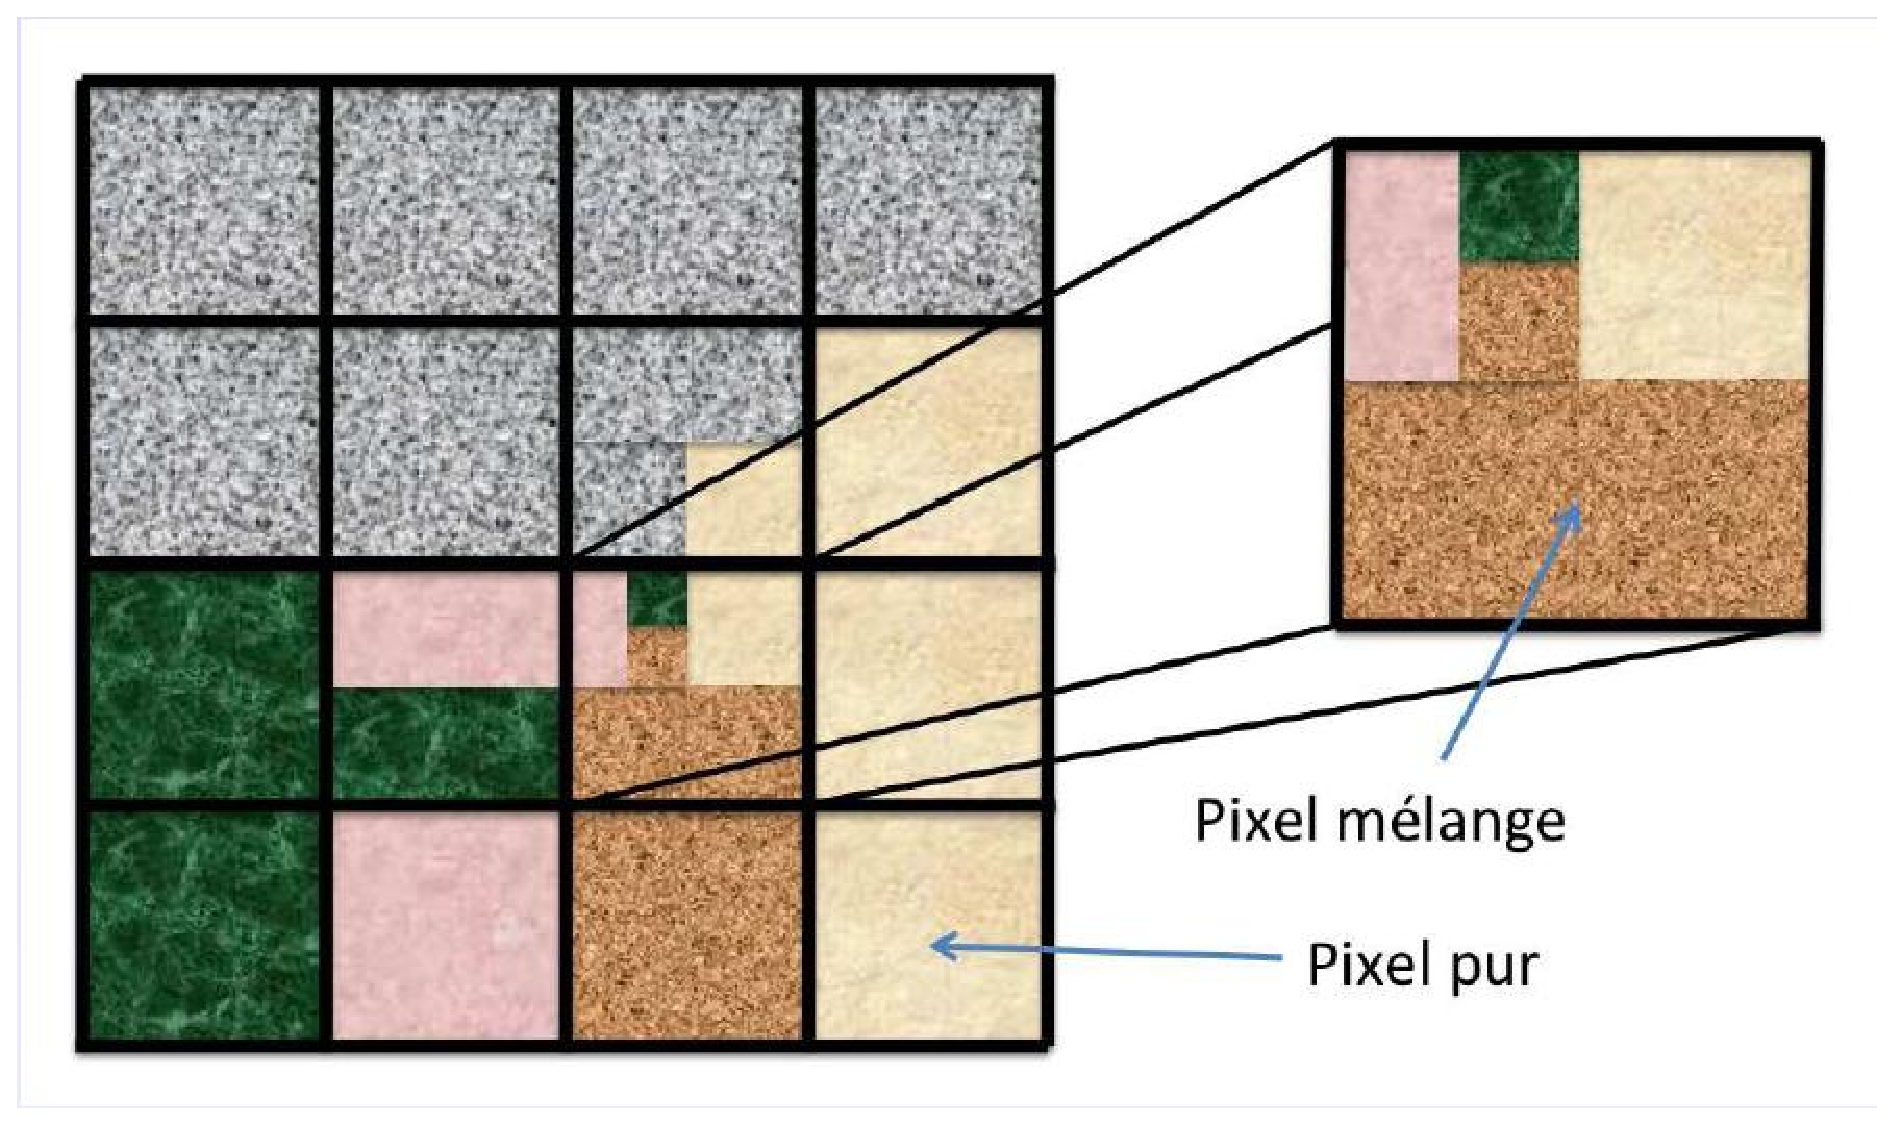
\includegraphics[width=0.7\textwidth]{Linear_Unmixing_HPX.eps}
  \itkcaption[Linear mixing model]{Zone which verify the LM model.}
  \label{fig:linear_unmixing}
\end{figure}

We notice \ref{fig:linear_unmixing} the
presence of pure pixels, and pixel-blending. The LMM acknowledges that
reflectance spectrum associated with each pixel is a linear combination of pure materials in the recovery area, commonly known as ``''endmembers. This is illustrated in \ref{fig:decomp_mml}

\begin{figure}[h]
  \centering
  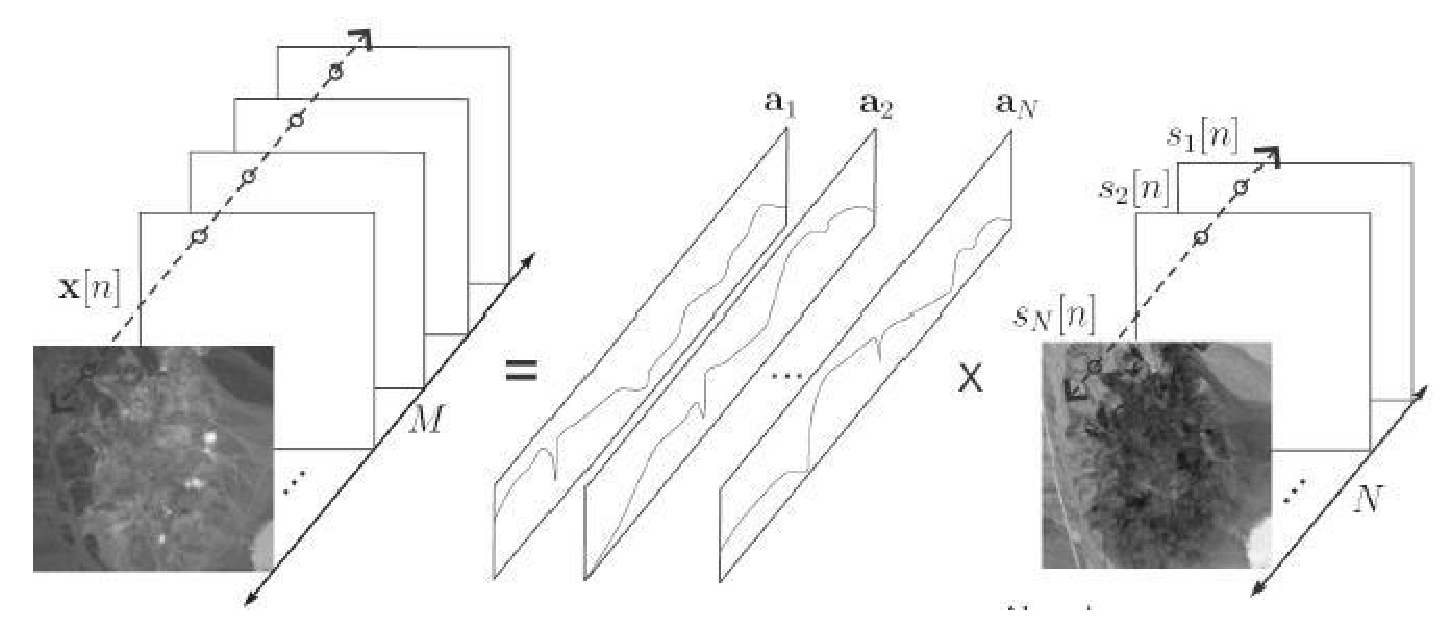
\includegraphics[width=0.7\textwidth]{Decomposition_MML_HPX.eps}
  \itkcaption[Decomposition of the LMM]{Decomposition of a hyperspectral cube according to the LMM.}
  \label{fig:decomp_mml}
\end{figure}
The `` left'' term represents the different spectral bands of
data cube. The `` right'' term represents a `` product''
between the reflectance spectra of endmembers and their repective abundances. Abundance band of endmembers is
image grayscale between $0$ and $1$. The pixel i of the
abundance band of endmember j is $s_ {ji}$. This value is the
abundance of endmember j in the pixel i. Under certain conditions
[Huck2009], this value can be interpreted as the ratio
surface of the material in the overlap zone (\ref{fig:linear_unmixing}). In
practice, one can reasonably expect that: 

\begin{itemize}
\item{a limit number
of pure materials compose the scene.}
\item{the scene contains pure pixels if the spatial resolution is sufficient and
do not necessarily contains them otherwise.}
\end{itemize}

Many techniques of unmixing in hyperspectral image analysis
are based on geometric approach where each pixel is seen as a spectral
vector of L (number of spectral bands). The
spectral bands can then be written as vectors.

\begin{figure}[h]
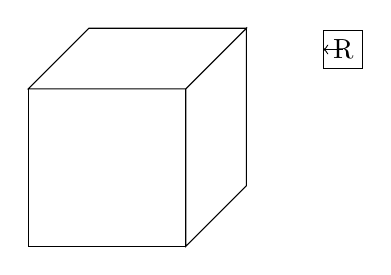
\begin{tikzpicture}
\pgfmathsetmacro{\cubex}{2}
\pgfmathsetmacro{\cubey}{2}
\pgfmathsetmacro{\cubez}{2}
\draw[black,fill=white] (0,0,0) -- ++(-\cubex,0,0) -- ++(0,-\cubey,0) -- ++(\cubex,0,0) -- cycle;
\draw[black,fill=white] (0,0,0) -- ++(0,0,-\cubez) -- ++(0,-\cubey,0) -- ++(0,0,\cubez) -- cycle;
\draw[black,fill=white] (0,0,0) -- ++(-\cubex,0,0) -- ++(0,0,-\cubez) -- ++(\cubex,0,0) -- cycle;
\node[draw] (R) at (2,0.5) {R};
\draw[->] (2,0.5) -- (R.west);
\end{tikzpicture}
\itkcaption[Hyperspectral cube vectorization]{``Vectorization'' of hyperspectral cube. The spectral pixels
are stored in the columns of the matrix R and, in
equivalently, the spectral bands are assigned to the lines of R.}
\label{fig:mml}
\end{figure}
%% Figure 5: "Vectorisation" du cube hyperspectral. Les pixels spectraux
%% sont ranges dans les colonnes de la matrice R et, de maniere
%% equivalente, les bandes spectrales sont rangees dans les lignes de R.

By deduction of \ref{fig:decomp_mml} et de \ref{fig:mml}, the LMM needs to decompose R as: 
\begin{center}
$R= A.S + N = X + N$
\end{center}

J is the number of endmembers and the number of spectral pixels I:
 
\begin{itemize}
\item{J columns of the matrix A contain the spectra of endmembers.}
\item{J rows of the matrix S contain the abundance maps
vectorized, we call the columns vectors of abundances of
matrix S.}
\item{The matrix N, of dimensions $LXI$ is a matrix of additive noise.}
\end{itemize}

The unmixing problem is to estimate matrices A and S
from R or possibly of \"X, an estimate of the denoised matrix signal.

Several physical constraints can be taken into
account to solve the unmixing problem:
 
\begin{itemize}
\item{C1: reflectance spectra are positives (non negative matrix A).}
\item{C2: positivity abundances are positive (non-negative matrix S).}
\item{C3: additivity
abundance (the sum of the coefficients of each column of the matrix S is 1).}
\item{Independence between the ``algebraic spectral vectors'' of endmembers associated with linearity and mixtures of spectra, so that the simplex property described in paragraph below.}
\end{itemize}

\subsection{Simplex}  
Recent unmixing algorithms based on the ``property of
simplex.'' In a vector space of dimension $J-1$, we can
associate to J vectors algebrically independent, J points which define the vertices of a J-simplex \ref{fig: simplex}.

\begin{figure}[h]
  \centering
  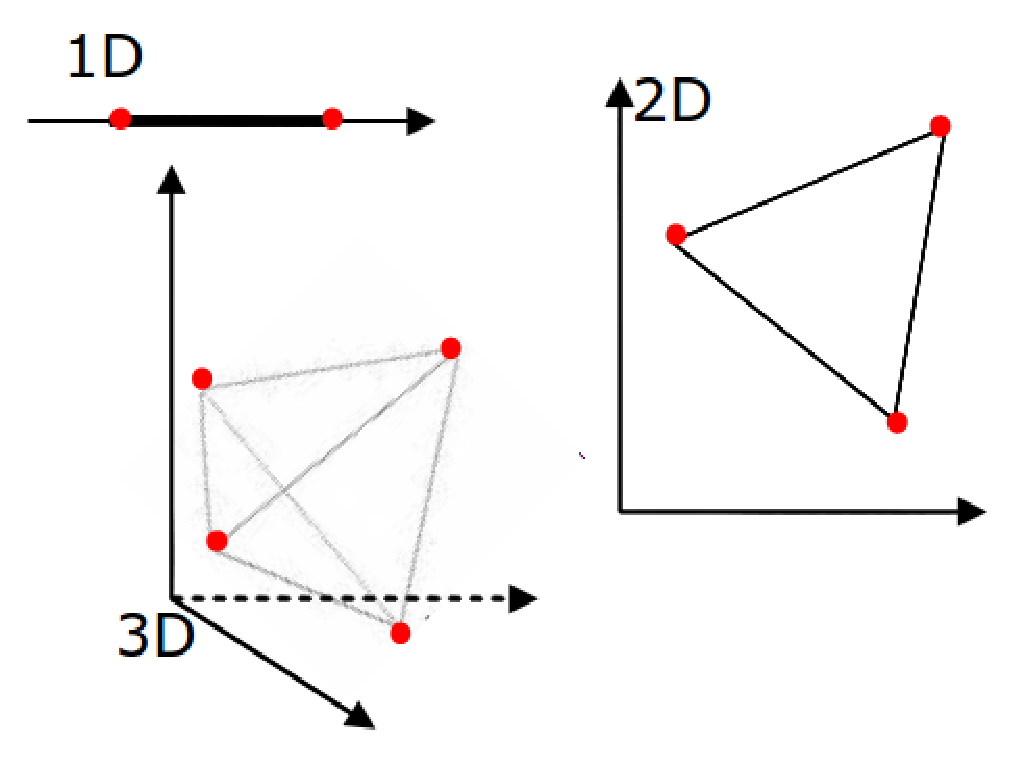
\includegraphics[width=0.7\textwidth]{Simplex_HPX.eps}
  \itkcaption[Simplex]{Illustration of a 2-simplex, a 3-simplex and a 4-simplex.}
  \label{fig:simplex}
\end{figure}

Hyperspectral cube of L bands, based on J endmembers,
may be contained in a affine subspace of dimension $J-1$.
A relevant subspace in the sense of signal-to-noise ratio is
generally obtained by Principal Component Analysis (PCA) \ref{sec:RoadExtraction}. 
In practice, the $J-1$ eigenvectors associated with highest values are
the columns of a projection matrix V of dimension $(Lx(J-1))$. Reduced
data Z, of dimensions $((J-1)xI)$ are obtained by the operation:
$Z=V^{T}(\tilde{R})$

where each column of $\tilde{R}$ where the average spectrum is substracted,
generally estimated under maximum likelihood. In the
subspace carrying the column-vectors Z, endmembers spectra oare associated to the top of the simplex. If the noise is
negligible, the simplex circumscribed reduced data.

This property shows that the endmembers research are the vertices of a
simplex that circumscribes the data. However, an infinity of different
simplices can identify the same data set. In fact, the problem of
unmixing generally does not have a unique solution. This degeneration can also be
demonstrated by the formalism of the non-negative
matrices factorization (see Huck2010a).

It is therefore necessary to choose the most physically
relevant solution. All unmixing techniques based on this simplex property admit that the best solution is defined by the allowable
minimum volume simplex, or the notion of volume is extended to all
finite dimensions (possibly different from 3).
  

\subsection{State of the art unmixing algorithms selection} 
The more recent linear unmixing algorithms exploit the
simplex property. It is possible to classify these methods into several families:

\subsubsection{Family 1} 
A first family of unmixing algorithms are based on research of the
endmembers ``among'' data. This means that a minimum of one pure pixel must
be associated with each endmembers. If this hypothesis is not
verified, it will produce an estimation error of the endmembers spectra. The historical advantage of these algorithms are their low
algorithmic complexity. The three best known are :
\begin{itemize}
\item PPI (Pixel Purity Index)
\item VCA NFINDER (Vertex Component Analysis) [Nascimento2005]
\end{itemize}

In addition to its success recognized by the
community and very competitive algorithmic complexity, the endmembers estimation is unbiased in absence of noise (and when there are pure pixels).

\paragraph{VCA} 
The VCA algorithm is systematically
used to initialize various studied algorithms (except
MVES, based on a different initialization).

Important elements on the operation of VCA:
\begin{itemize}
\item {The VCA algorithm
is based on iterative projections of the data orthogonal to
the subspace already held by the endmembers.}
\item {Biaised when degree of purity is lower than 1.}
\end{itemize}  

\subsubsection{Family 2} 
A second family is composed of algorithms which are looking for the simplex of minimum
volume circumscribing the data. Phase initialization consists in determining
an initial simplex any circumscribing the data. Then, a numerical
optimization scheme minimizes a functional, increasing function of the
volume generalized, itself dependent of estimated endmembersin the
current iteration. The optimization scheme is constrained by the fact that the
data have remained on the simplex and possibly by constraints C1, C2 and C3.

Existing algorithms are: 
\begin{itemize}
\item {MVSA (Minimum Volume Simplex
Analysis) [Li2008].}
\item { MVES (Minimum Volume Encosing Simplex)
[Chan2009].}
\item {SISAL (Simplex Identification via Split Augmented
Lagrangian) [Dias2009].}
\end{itemize}  
  
Main differences between algorithms are: 
\begin{itemize}
\item {The numerical optimization scheme.}
\item {The way
constraints are taken into account.}

\end{itemize}  
These issues impact the computational complexity and the precision of the estimation.
 
\paragraph{MVSA aLi2008]} 
MVSA key points: 
\begin{itemize}
\item {Initialization by VCA.}
\item {All spectral pixels included in the simplex estimate
  (approximatively) by VCA does not impact the constraint of  data to belong to the researched simplex, they are
  simply delete the data used in the minimization of the
  simplex to reduce the algorithmic complexity.}
\item {The highly developed optimization technique uses
  sequential quadratic programming (Sequential Quadratic
  Programming - SQP) and more specifically of the category
  ``Quasi-Newton''under constraint.}
\end{itemize} 

\paragraph{MVES [Chan2009]}
 MVES key points: 
\begin{itemize}
\item {Initialization by non-trivial
  iterative method (LP Linear Programming for Linear
  Programming), different from VCA.}
\item {Resolution of problem by LP.}
\end{itemize} 
 

\paragraph{SISAL [Dias2009]}
SISAL key points:
\begin{itemize}
\item {Initialisation by VCA.}
\item {Selection of similar spectral pixels as MVSA to reduce computational complexity.}
\item {Advanced optimization technique
combining multiple features.}
\begin{itemize}
\item {Decomposition of the non convex problem
in convex set of problems.}
\item {Development of a
specific method of separation of variables for considering
Lagrangian increases with a good design properties.}
\end{itemize}
\end{itemize} 

\subsubsection{Family 3}
Non negative matrix factorization algorithms (NMF for Non-negative Matrix Factorization). The purpose of this
branch of applied mathematics is to factor a non-negative matrix, X in our case, into a product of non negative matrices: AS by minimizing a distance between X and AS and
with an adapted regularization to lift the degeneration in an appropriate manner adapted to the physical problems associated with unmixing.

\paragraph{MDMD-NMF [Huck2010b]} 
Key points of MDMD-NMF:
\begin{itemize}
\item {VCA initialization.}
\item {Minimizing the norm of standard
Frobenius with a spectral regularization and a regularization ``Space''(the matrix of abundances).}
\begin{itemize}
\item {Minimum spectral
Dispersion: the spectral regularization encourages the  variance of 
coefficients of a spectrum of endmembers to be low.}
\item {Maximum spatial dispersion: the spatial regularization
  encourages the vector of abundances to occupy all the admissible parts (more information in [Huck2009]). it
  presents a certain analogy with the minimum volume constraint.}
\end{itemize}
\end{itemize}
 
 
  

\subsubsection{Remarques complementaires}
Les algorithmes des familles 1 et 2 estiment les spectres de
endmembers ``seulement''. L'estimation des cartes d'abondances a lieu
a posteriori et requiert l'application d'un algorithme de type Fully
Constrained Least Square (FCLS) [Heinz2001]. MVES inclut un algorithme
specifique d'estimation des abondances, que nous avons utilise dans
nos simulations (pour MVES seulement).  
Le demixage est un probleme generalement non convexe, ce
qui explique l'importance de l'initialisation des algorithmes.
Recapitulatif de la prise en compte des differentes contraintes
physiques:


\begin{center}
   \begin{tabular}{ l | l | l | l | l | l }
     \hline
     & VCA & MVSA & MVES & SISAL & MDMD \\ \hline
     C1 $(A>0)$ & muette & Muette & Muette & Muette & Dure \\ \hline
     C2 $(S>0)$ & muette & Dure & Dure & Souple & Dure \\ \hline
     C3 (additivite) & Muette (via FCLS) & Dure & Dure & Dure & Souple \\ \hline
     simplexe & Endmembers \newline parmi les donnees & Circonscrit \newline aux donnees & 
     Circonscrit \newline aux donnees & Circonscrit \newline aux donnees &
     Indirecte par la \newline regularisation ``spatiale'' \\ \hline
   \end{tabular}
 \end{center}

\section{Dimensionality reduction}

\section{Anomaly detection}
Une anomalie dans une scene est, par definition, un element qu'on ne
s'attend pas a y trouver. L'element anormal est donc de nature
differente de son environnement et sa presence est minoritaire dans la
scene. Typiquement, un vehicule dans en milieu naturel, un rocher dans
champ, une cabane en bois dans une foret suffisamment clairsemee sont
autant d'anomalies que l'on peut souhaiter detecter a l'aide
d'imagerie hyperspectrale. Cela suppose que la reponse spectrale de
l'anomalie puisse etre discriminee de la reponse spectrale du
``fouilli-du-fond'' (background clutter). Cela suppose egalement que
les pixels associes aux anomalies, les pixels anormaux, sont
suffisamment rares et/ou ponctuels pour pouvoir etre consideres comme
tels. Ces proprietes peuvent etre vues comme des hypotheses spectrales
et spatiales sur lesquelles s'appuient les techniques de detection
d'anomalies dans les images hyperspectrales.

Nous rappelons que la litterature relative a l'imagerie hyperspectrale
distingue generalement la detection de cibles et la detection
d'anomalies:

\begin{itemize}
\item {On parle de detection de cibles lorsque la reponse
spectrale de l'element recherche est utilisee en entree de
l'algorithme de detection. Il s'agit d'information a priori qui
permet, en theorie, de construire des algorithmes a tres fort pouvoir
de detection, tels que l'Adaptive Matched Filter (AMF) ou l'Adaptive
Cosine/Coherence Estimator (ACE),pour n'en citer que deux. Neanmoins,
la connaissance suffisamment fine du spectre recherche est une
information difficile a detenir en pratique, ce qui conduit bien
souvent a l'utilisation d'algorithmes de detection d'anomalies.}
\item {On parle de detection d'anomalies lorsque le spectre de
  l'element anormal n'est pas requis par l'algorithme de
  detection. Pour cette raison, on associe souvent le terme de
  ``detection non supervisee''. Neanmoins, les algorithmes dependent
  generalement de ``parametres de structure''. Par exemple, dans le
  cas de la detection dans une fenetre glissante, le juste choix des
  dimensions repose sur une connaissance a priori de la taille des
  anomalies recherchees. Cette partie de l'etude se concentre sur la
  comparaison d'algorithmes de detection d'anomalies.}
\end{itemize}
    
\begin{figure}[h]
  \centering
  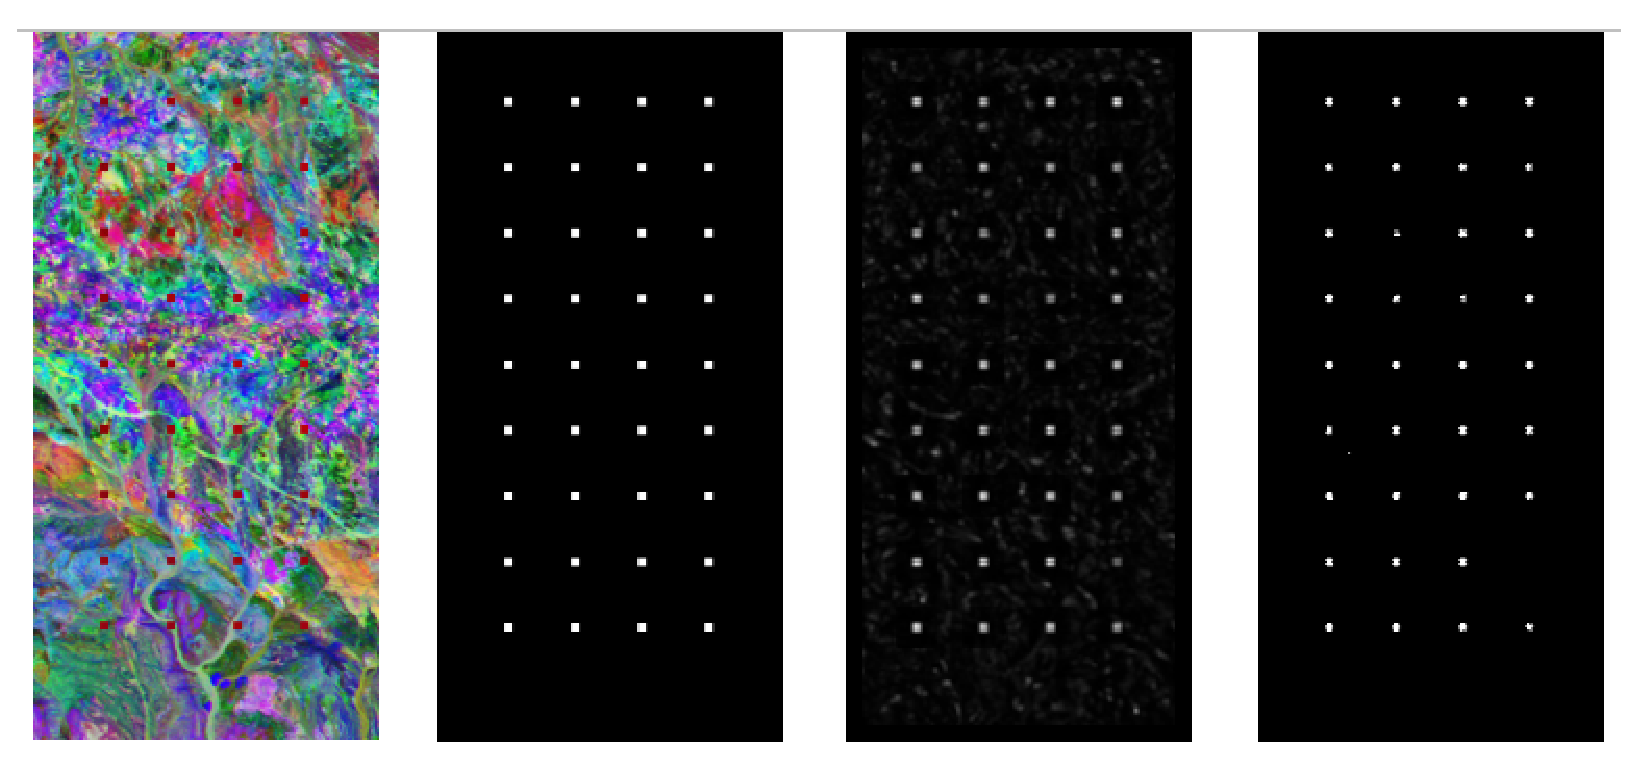
\includegraphics[width=0.7\textwidth]{Anomaly_HYP.eps}
  \itkcaption[Notion sur la detection]{Notions sur la detection: masque de verite terrain, carte de detection, masque de detection.}
  \label{fig:anomaly_hyp}
\end{figure}
In \ref{fig:anomaly_hyp}, nous introduisons d'ores et deja quelques notions
qui seront utiles par la suite. Les algorithmes de detection
d'anomalies ont comme entree une image et estiment une carte de
detection faisant office d'outil d'aide a la prise de decision. Un
seuillage adapte permet d'obtenir un masque de detection estime, que
l'on espere le plus ressemblant possible au masque de verite terrain,
inconnu en pratique. Ce masque estime a la vocation d'un outil de
prises automatiques de decisions.

Deux approches dominent l'etat de l'art sur la detection d'anomalies
dans les images hyperspectrales. Il s'agit des methodes par Poursuite
de Projection (PP) et les methodes basees sur une modelisation
probabiliste de la classe fond et eventuellement de la classe cible
avec test d'hypotheses statistiques.
La PP consiste a projeter lineairement les pixels spectraux sur des
vecteurs wi qui optimise un critere sensible a la presence d'anomalies
(ex: kurtosis). On obtient une serie de cartes de projections ou les
anomalies contrastent tres fortement avec le fond. Mais l'estimation
automatique d'une carte de detection presente des difficultes
majeures, notamment:
\begin{itemize} 
\item Combien de projecteurs doit-on estimer?  
\item Quel(s) projecteur(s) choisir?  
\item Comment gerer un fond inhomogene?  
\item Les performances de detection varient avec les dimensions spatiales de l'image (nombre d'echantillons) 
\item Ces algorithmes ont generalement une structure peu parallelisable
\item Ces algorithmes ne sont generalement pas ``a taux de fausse alarme constant''.
\end{itemize}

Les algorithmes selectionnes sont RX (presente en premiere version
dans [Reed1990] et GMRF [Schweizer2001] et leurs specificites
respectives seront presentees plus loin. Ils sont bases sur les
notions de modeles probabilistes, test d'hypotheses statistiques et
fenetre glissante.  Ce type d'approche consiste a repondre a la
question: ``Le pixel (ou ensemble de pixels voisins) teste
ressemble-t-il au pixels du fond?'' par une demarche de test
statistique. De maniere plus exhaustive, cette demarche necessite:
\begin{itemize} 
\item Un modele pour la classe ``fond'' 
\item Le choix d'un test statistique 
\item Eventuellement, un modele pour la classe ``anomalie''
\item Des estimateurs pour les differents parametres inconnus a priori
\item Des hypotheses d'homogeneite permettant un compromis satisfaisant entre: 
\begin{itemize} 
\item Le nombre d'echantillons en regard du nombre de parametres a
  estimer 
\item L'homogeneite, notamment du fond 
\item La complexite algorithmique (quoique les algorithmes consideres sont
hautement parallelisables)
\end{itemize} 
\end{itemize} 
Le principe de fonctionnement de RX et GLRT peut etre resume par les
Figure 27  et Figure 28.
(TODO do block diagramme using tikz)

Une premiere etape facultative (spontanement consideree dans le cadre
de cette etude) consiste a reduire la dimension spectrale des donnees
tout en conservant l'information liee aux anomalies. Puis, les pixels
spectraux sont testes a tour de rôle (tache parallelisable). Le pixel
teste se voit attribuer une fenetre glissante (voir Figure 28). Cette
fenetre comprend deux sous fenetres, centrees sur le pixel teste, de
dimensions respectives L et LL, avec $L < LL$. 
\begin{itemize}
\item Les pixels appartenant a la couronne ainsi formee appartiennent
  a la classe ``fond local''. Les parametres statistiques du fond,
  requis par les tests statistiques, sont estimes a partir de ces
  pixels spectraux. L'une des difficultes consiste a trouver un
  compromis sur l'epaisseur de la couronne (et donc le nombre
  d'echantillons statistiques) sachant que: 
\begin{itemize}
\item Si la couronne est trop epaisse, le fond local n'est plus
  suffisamment homogene 
\item Si le nombre d'echantillons est trop faible, la precision de
  l'estimation statistique des parametres du modele du fond est trop
  faible
\end{itemize}  
\item Les pixels de la partie centrale de la fenetre glissante
  appartiennent a la classe ``inconnue''. Si le pixel teste (pixel
  central) est un pixel anormal, il est possible que ses voisins
  soient aussi des pixels anormaux, d'ou l'interet de ne pas choisir
  une valeur de L trop faible si l'on sait que les anomalies
  recherchees peuvent etre reparties sur plusieurs pixels.
\end{itemize}  
Une fois l'ensemble des
parametres estimes, un test statistique est effectue et affecte une
valeur $\Lambda(i)$ au pixel teste i. Une carte de detection est ainsi
constituee.

Figure 28: Principe de la fenetre glissante et definitions des
parametres L et LL de la fenetre glissante.  Les algorithmes RX et
GMRF, consideres dans presentes dans les sections suivantes.
(TODO  block diagram for windowing using tikz)

\subsection{Local RX}
